
	\section{Conditional probability}
In general, our evaluation of the probabilities changes if our state of information changes. If we observe that the sky is cloudy, our evaluation of the probability that it will rain will become greater. Given an event $E$, if $\mathbb P(\cdot )$ denotes the probability before the knowledge of $E$, we will denote the new probability, given the knowledge of $E$, by $\mathbb P( \cdot |E)$. With this notations, the previous example reads $\mathbb P(\text{"Today it will rain "}|\text{"It is cloudy"}) > \mathbb P(\text{"It will rain today "})$. In case the \emph{ conditioning } event $E$ can be written in terms of the sample space, that is, in case $E \subset \Omega$, $\mathbb P(\cdot |E)$ can be described in simple terms. 	

%%%%%%%%%%%%%%%%%%%%%%%%%%%%%%%%%%%%%%%%%%%%%%%%%%%%%%%%%%%%%%%%%%%%%%%%%%%%%%%%%%%%%%%%%%%%%%%%%%%%%%%%%%%%%%%%%%%%%%%%%%%%%%%%%%%%%%%%%%%%%%%%%%%%%%%%%%%%%%%%%%%%%%%%%%%%%%%%%%%%%%%%%%%%%%%%%%%%%%%%%%%%%%%%%%%%%%%%%%%
%%%%%%%%%%%%%%%%%%%%%%%%%%%%%%%%%%%%%%%%%%%%%%%%%%%%%%%%%%%%% DEFINITION OF CONDITIONAL PROBABILITY %%%%%%%%%%%%%%%%%%%%%%%%%%%%%%%%%%%%%%%%%%%%%%%%%%%%%%%%%%%%%%%%%%%%%%%%%%%%%%%%%%%%%%%%%%%%%%%%%%%%%%%%%%%%%%%%%%%%%%%
%%%%%%%%%%%%%%%%%%%%%%%%%%%%%%%%%%%%%%%%%%%%%%%%%%%%%%%%%%%%%%%%%%%%%%%%%%%%%%%%%%%%%%%%%%%%%%%%%%%%%%%%%%%%%%%%%%%%%%%%%%%%%%%%%%%%%%%%%%%%%%%%%%%%%%%%%%%%%%%%%%%%%%%%%%%%%%%%%%%%%%%%%%%%%%%%%%%%%%%%%%%%%%%%%%%%%%%%%%%

	\subsection{Definition and first examples }
	Let $\Omega=\{\omega_1,...,\omega_n\}$ be the sample space, $\mathbb P$ a probability over $\Omega$, see Definition~\ref{d:prob3}, and let $B \subset \Omega$ be an event.
	%\sidenote{Here we are assuming that the event we observe can be written in terms of our elementary events. Thus, in general, you should refine your sample space to contain the event you observe } 
	The probability \emph{conditioned to B} is a new probability denoted by the symbol $\mathbb{P}(\cdot| B) $. Intuitively, it has to satisfy that
	\bel{e:cond1}{
		\mathbb P((\{\omega\}| E) = 0 \qquad \text{if $\omega \notin E$ }
	}
	and, since we do not have information on which event $\omega \in E $  caused $E$, we would like to maintain the proportions 
	\bel{e:cond2}{
		\mathbb P(\{\omega\}|E) = C \mathbb P(\{\omega\}) = Cp_\omega,
	}
	for some constant $C$. The constant $C$ is to be determined by \eqref{e:normalization}: 
	\bel{e:cond3}{
		1 = \sum_{\omega \in \Omega} \mathbb P(\{\omega\}|E ) = \sum_{\omega \in E} C \mathbb P(\{\omega\})  = C \mathbb P(E)
	}
	so that $ C = \mathbb P(E)$. 
	For the sake of concreteness we rewrite \eqref{e:cond3} using a different and extended notation. Let $E = \{\omega_{i_1}, \ldots , \omega_{i_k}\}$, for some $k \in \mathbb N$ and $1 \leq i_1 < \ldots < i_k \leq n$ be an event, then 
	\bel{e:cond4}{
		1 &= \mathbb P(\{\omega_1, \ldots, \omega_n\}| \{\omega_{i_1}, \ldots , \omega_{i_k}\}) \\ 
		& = \sum_{i = 1}^n \mathbb P(\{\omega_i\}|\{\omega_{i_1},\ldots, \omega_{i_k}\})  = C \sum_{j =1}^k\mathbb P(\{\omega_{i_j}\}) = C \mathbb P(E) 
	}
	Therefore $C = \frac{1}{\mathbb P(E)}$ and the probability of an ev
	
	that is, we denote the probability of $A$ conditioned to $B$ by $\mathbb{P}(A|B)$. Of course, the new probability has to satisfy  $\mathbb{P}(\omega|B)=0$ if $\omega\notin B$. If $\omega\in B$, what should the new value $\mathbb{P}(\omega|B)$ be? Since the new information tells us only that $B$ is true, but it does not give us information about the single $\omega$s in $B$, the proportions given by $\mathbb{P}$ in $B$ should be maintained by $\mathbb{P}(\cdot|B)$.  Therefore we set $\mathbb{P}(\omega|B)=c\mathbb{P}(\omega)$ if $\omega\in B$, for some constant $c$. $c$ which can be determined by requiring $\mathbb{P}(\cdot|B)$ has to satisfy \eqref{e:fun}. If $B=\{\omega_1,...,\omega_k\}$, we obtain that 
	\bel{}{1 & =\mathbb{P}(\omega|B)+...+\mathbb{P}(\omega_k|B)+\mathbb{P}(\omega_{k+1}|B)+...+\mathbb{P}(\omega_n|B)
	\\ &=c\mathbb{P}(\omega_1)+...+c\mathbb{P}(\omega_k)=c(\mathbb{P}(\omega_1)+...+\mathbb{P}(\omega_k))=c\mathbb{P}(B).
	}
	Therefore $c=1/\mathbb{P}(B)$ and
	
	\bel{e:condi}{
	\mathbb{P}(\omega|B)=
		\begin{cases}
		\frac{\mathbb{P}(\omega)}{\mathbb{P}(B)} & \textrm{ if }\omega\in B\\
		0 & \textrm{ if } \omega \notin B,
	\end{cases}
	} 
	
	Considering an event $A=\{\omega_1,...,\omega_s,\omega_{k+1},...,\omega_{k+m}\}$, where $s \leq k$ formula \eqref{d:prob}  leads to \bel{}{\mathbb{P}(A|B)=\frac{\mathbb{P}(\omega_1)+....+\mathbb{P}(\omega_s) }{\mathbb P (B)}= \frac{\mathbb{P}(A \cap B)}{\mathbb{P}(B)}}
	
	\begin{definition}
	\label{conditional}
		Let $\Omega$ be the sample space and let $\mathbb{P}$ be a probability. Consider an event $B\subset \Omega$ such that $\mathbb{P}(B)>0$. The conditional probability $\mathbb{P}(\cdot |B)$ given $B$ is the probability measure defined by   
		\bel{}{\Omega \supset A \mapsto \mathbb{P}(A\vert B):= \frac{\mathbb{P}(A\cap B)}{\mathbb{P}(B)}, }
		that is, is the probability that associates to each $A \subset \Omega$ the value $\mathbb \mathbb P(A|B) = \mathbb P(A \cap B )/ \mathbb P(B)$.
	\end{definition}
	
	As shown in Figure ~\ref{fig:cond_prob}, there is an easy interpretation of the conditional probability. Recall from ??? that one can interpret a probability as a way of measuring areas (in the discrete setting as a way to count which gives different weights to different events). If we observe $B$, our new evaluation of the area doesn't change in $E$ and outside $E$ is updated set zero. Since one of the conditions imposed to a probability is that the total area is 1, see Proposition~\ref{p:}, to maintain this property we need to divide the new evaluation by $E$. In this sense we maintain the proportions of our evaluations inside $E$ (since we do not have any information on which event caused $E$) and we set them to 0 outside, since we know that $E$ happened.  Alternative, one can think that we are redistributing the mass of $E^c$, that is $\mathbb P(E^c)$, to $E$, in such a way that the proportions do not change. 
	\begin{figure}
	 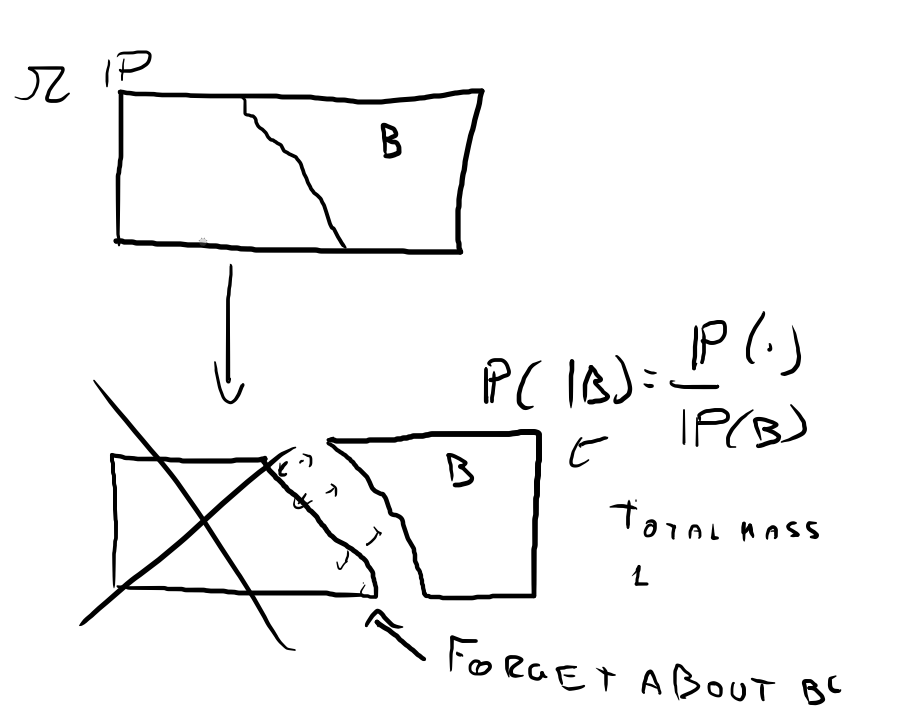
\includegraphics[width = 10cm]{Conditional_Probability.png}
	    \caption{We forget about $B^c$ and we consider $\mathbb P$ restricted to subsets of $\mathbb B$. However, to obtain total mass 1 without favouring any of the $\omega \in B$, we multiply by $\frac{1}{\mathbb P(B)}$.  }
	    \label{f:cond_prob}
	    \end{figure}
	    One can think at a probability as a distribution of a mass, which in total is 1, over $\Omega$. If one takes the distribution of mass given by $\mathbb P$ and sets the mass of $ B^c$ to be zero, one has a distribution of mass whose total is not 1. In order to obtain the distribution of mass given by the conditional probability $\mathbb P(\cdot | B)$, one has therefore to redistribute the mass it has removed, $\mathbb P(B^c)$, in such a way to not change the relative masses of the singletons in $B$. Thus $\mathbb P(\omega|B) = \mathbb P(\omega) + \mathbb P(\omega) \mathbb P(B^c)/\mathbb P(B)$. This way of thinking can be useful for the Exercise  ~\ref{e:conditional_samplig}. 
	Note also that  Example \eqref{e:Judicial} and  Exercise \eqref{e:Harvard} show that probabilities can vary a lot if conditioned to the an event $B$. This is schematically shown in Figure \eqref{fig:prop} 
	\begin{figure}
	 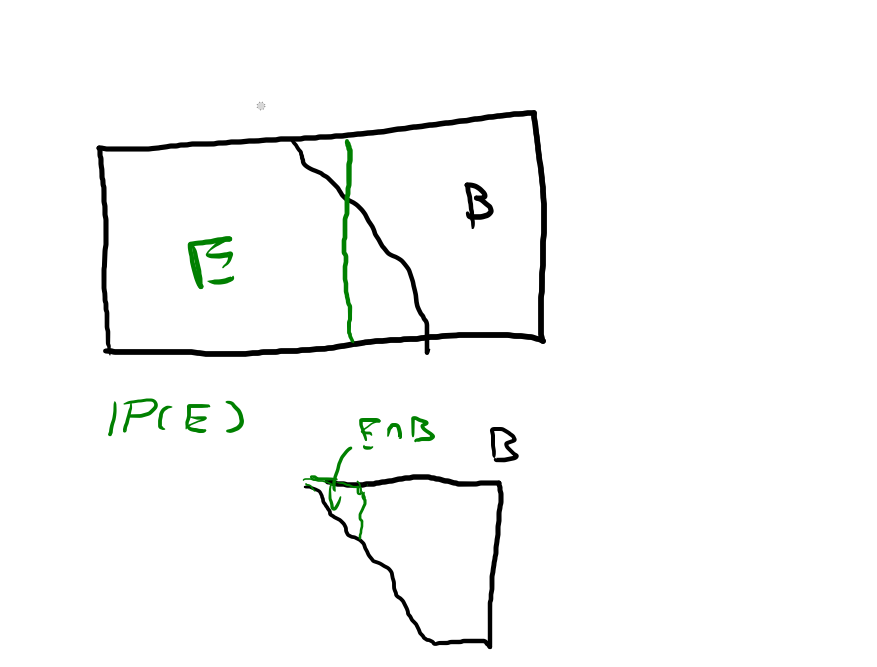
\includegraphics[width =10cm]{Proportion_conditional.png}
	    \caption{$\mathbb P(E)$ is much greater that $\mathbb P(E|B)$. }
	    \label{fig:prop}
	    \end{figure}
	    
	\begin{ExerciseList}
		\Exercise We throw two dice and assume that each of numbers is equally probable \sidenote{In other words, on $\Omega$ we assume that $\mathbb P$ is the uniform one. Why this is the case  investigated in Subsection\ref{ss:independence}} what is the probability conditioned on "The sum of the two dice is 7"?.
	
	% \Answer The sample space is $\Omega=\{(i,j)\,,\,i,j\in\{1,2,3,4,5,6\}\}$, and the event corresponds to $B=\{(1,6),(2,5),(3,4),(4,3),(5,2),(6,1)\}$. We see  that $\mathbb{P}(\omega|A)=\frac{1/36}{6/36}=1/6$ if $i+j=7$, $0 $ otherwise. That is,all the outcomes in $A$ are equally probable on the new sample space $\Omega =\{(i,j)\, i,j \in \{1,2,3,4,5,6\}\,\,i+j = 7\}$. 
		
	
	
		\Exercise You toss a fair coin independently 4 times \footnote{The same remark applies here: the probability is the uniform one and in Subsection \ref{ss:independence} we will see why}. Show that, knowing that only one head has been observed, the head is equally probable to have appeared in the 1st,2nd,3rd and 4th position.  
	
	    \Answer 
	
	    The sample space is $\Omega = \{0000,0001,0010,\ldots, 1111\}$. Let $B = =\{x_1x_2x_3x_4\,,\, x_1 + x_2 + x_3 + x_4 = 1 \} = \{1000,0100,0010,0001\}$ be the event that only one heads result has shown up. 
	    The probability of the singleton $x_1x_2x_3x_4$, where $x_i \in \{0,1\}$ for $i =1,2,3,4$, conditioned to $B$ is given by 
	    $$
	    \mathbb P(x_1x_2x_3x_4| B) = 0
	    $$
	    if $x_1 + x_2 + x_3 + x_4 = 1 $
	    and is equal to 
	    $$
	    \mathbb P(x_1x_2x_3x_4|B) = \frac{1/2^4}{4/2^4} = 1/4,
	    $$
	    which is to say that there is not favourite position in which the heads might appear. 
	
	    
		\Exercise
	Let $\Omega = \{\omega_1,...,\omega_n\}$ be a sample space and let $\mathbb P$ be a probability assigned to it. Let $B \subset \Omega$ be an event, and assume $\mathbb P(B) > 0$.       \Question Prove that $\mathbb P(\cdot |B)$ is a probability on the sample space $B$. 
	\Question Assume that $\mathbb P$ is the uniform probability defined in \eqref{e:unif} on $\Omega$. Show that  $\mathbb{P}(\cdot | B)$ is the uniform probability on the new sample space $B$.
	
	
	    \Answer 
	
	    \Question In order to show that $\mathbb P(\cdot | B)$ is a probability measure, we have to show that 
	    \begin{itemize}
	        \item $\mathbb P(\omega| B) \in [0,1]$\\
	        \item (\eqref{e:fun} holds)$\sum_{\omega \in B } \mathbb P(\omega | B) =1$ \\
	        \item (\eqref{d:prob} holds) For each $F \subset B$, $\mathbb P(F|B) = \sum_{\omega \in F } \mathbb P(\omega |B)$.
	    \end{itemize}
		   The first condition is true since, if $\omega \in B$, $\mathbb P(\omega) \leq \mathbb P(B)$, and therefore $\mathbb P(\omega | B) = \mathbb P(\omega)/\mathbb P(B) \leq 1$. The second condition, which can be rewritten by Proposition \eqref{p1} as  
	    $$
	    \mathbb P (B | B ) = 1
	    $$
	    is true since $$
	    \mathbb P(B | B) = \frac{\mathbb P(B \cap B)}{ \mathbb P(B)} = 1. 
	    $$
	    The last condition is true since 
	    \bel{}{
	    \mathbb P(F| B) = \frac{\mathbb P(F \cap B )}{\mathbb P(B)} = \frac{\mathbb P(F)}{\mathbb P(B)}\\ 
	    \sum_{\omega \in F } \frac{\mathbb P(\omega)}{\mathbb P(B)} = \sum_{\omega \in F} \mathbb P(\omega | B ).
	    }
	    \Question  As for the second question, since we have just proved that $\mathbb P$ is a probability measure on $B$, it suffices to note that every elementary event has the same probability (recall how we have derived formula \eqref{e:unif}: simply by assuming that the probability was equal on each elementary event). In fact $\forall \omega \in B$ $\mathbb P(\omega| B) = \mathbb P(\omega)/ \mathbb P(B)$ does not depend on $\omega$,  since by assumption  $\mathbb P $ does not depend on $\omega$.
	    
	    \Exercise (\cite{Feller}, Chapter V.8) Three dice are rolled. If no two show the same face, what is the probability that one is an ace?
	
		\Answer The sample space is $\Omega=\{(i,j,k)\,,i,j,k\in \{1,....6\}\}$, and the event "No two dice show the same face is $A=\{(i,j,k)\in \Omega\,,\, i\neq j, j\neq k, i\neq k\}$. The event B="The sum of the two dice is 7" is such that  $A \cap B$ is the disjoint union of the events"A and the 1 is in 1st position", "A and the 1 is in 2nd", "A and the 1 is in 3rd poosition". This union is disjoint since if $A$ happens, a 1 in the 1st position implies that there is no 1 neither in the 2nd nor in the 3rd. In formulas $A\cap B =( A\cap B_1) \cup (A \cap B_2) \cup (A \cap B_3)$, where $B_1 = \{(1,j,k)\in \Omega\}$, $B_2 =\{(i,1,k)\in \Omega\}$ and $B_3 = \{(i,j,1)\in \Omega\}$.  Thus 
	
	\bel{}{\mathbb{P}(B|A) & = \frac{\mathbb{P}(A \cap B)}{\mathbb{P}(B)} = \frac{\mathbb{P}(A \cap B_1)}{\mathbb{P}(A)} \\
		 & + \frac{\mathbb{P}(A \cap B_2)}{\mathbb{P}(A)} + \frac{\mathbb{P}(A \cap B_3)}{\mathbb{P}(A)}= 3\frac{\mathbb{P}( A \cap B_1)}{\mathbb{P}(A)}. }
		The event $A \cap B_1= \{(1,j,k)\, ,\, j\neq k\}$  is composed by $6\times 5 =30$ elements.  The event $A$ is composed by $ 6 \times 5 \times 4 $ elements.  Thus  
		\bel{}{\mathbb{P}(B|A)=\frac{6\times 5/216}{6\times 5 \times 4/216 }=\frac{6\times 5 }{6\times 5 \times 4}=1/4}
	
	
	\Exercise Consider an urn containg 2 blue marbles, 1 green marble and 1 red marble. Draw randomly (with uniform probability) one of them. 
	    \Question What is the probability of extracting a red marble if you know that the extracted marble is not green? 
	    \Question We do the following procedure. We draw a marble uniformly. If it is red we draw another marble independently, if not we finish the procedure. We are interested in the colour of the extracted marble: what is the probability of extracting a red marble?  	
	    \Question Note that it is not necessary to know the probability of drawing in one draw the red ball, that is $\mathbb P(r)$. Note also that in the second exercises gives you a procedure to draw from a bowl where you have removed the red marbles, even if you are drawing from a bowl that has them. 
	    \Answer 
	        \Question The sample space is $\Omega =\{ r,b,g\}$,$\mathbb P(r) = 1/4$, $\mathbb P(b) = 1/2$ and $ \mathbb P (g) = 1/4$. Thus $$
	        \mathbb P(g^c | r^c) = \frac{\mathbb P(b)}{\mathbb P({b,g})} 
	         = \frac{2}{3}
	        $$
	        \Question Now the sample space is more complicated, and resembles the game of Exercise ~\eqref{e:game} 
	        $$
	        \Omega = \{r...rc_{n}\,,\, n \in \mathbb N\,,c_n \in\{b,g\}\} \cup \{rr...\}
	        $$
	        The probability that we place in $\Omega$ is the following: The infinite sequence has probability 0: $\mathbb P\left(r...\right)$, while the finite sequences have probability 
	        \bel{}{
	          \mathbb P(rr...rc_{n}) = \mathbb P(rr...rc_{n}|\textrm{"first extraction r"}) \mathbb P(r) =  \mathbb P(r...c_{n-1})\mathbb P(r) \\
	          =...= \mathbb P(r)^{n-1} \mathbb P(c_{n})
	         }
	         (It will be maybe more clear once the geometric random variable has been obtained)
	         and we take $\mathbb P(c) =$(number of balls of colour c)/(total number of balls). 
	         The event I draw a blue ball is 
	         the event $\{ b,rb,rrb,...\}$
	         which has probability 
	         \bel{}{
	         \mathbb P(\textrm{"I draw a blue ball"}) & = \mathbb P(b) + \mathbb P(b)\mathbb P(r) + \mathbb P(b)\mathbb P(r)^2+ \ldots\\
	          & = \mathbb P(b)\left(\sum_{i = 0}^{+ \infty} \mathbb P(r)^i \right) = \frac{\mathbb P(b)}{1- \mathbb P(r)} = \frac{\mathbb P(b)}{\mathbb P(b) + \mathbb P(g)} = 2/3 
	          }
	         \Question The above procedure can be used to draw on a bowl of. In a more realistic situation, maybe you want to interview families with children, but you don't have at disposal the "bowl", that is, the list with of the families of two children. This exercises tells that it suffices to contact each family untill a family with children is contacted. In more complex situations (i.e, in montecarlo simulations), a similar method is used to get to know the conditional probabilities  
	
	\end{ExerciseList}
	
		\begin{example}[Sampling interpretation of the Conditional Probability]
	
	Suppose that the Italian population  is composed by $N$ individuals, that $N_B$  of them are taller than 175 cm and that $N_A$ of them come from Sardinia. Let the events that a person chosen at random (i.e. with uniform probability) is taller than 175 cm and a comes from Sardinia be A and B, respectively.
	Then $\mathbb{P}(A) = N_A/N$ and $\mathbb{P}(B|A)=N_{AB}/N_{A}$, where $N_{AB}$ is the number of people coming from Sardinia being taller than 175 cm. The interpretation of the probability measure $\mathbb{P}(\cdot|A)$ is clear: we are extracting a random person from the subpopulation $N_A$ (which is a population on its own right), the one composed by people from Sardinia . 
	
	\end{example}
	
	\textbf{A judicial case}
	\label{e:Judicial}
	A woman had been killed, and the principal suspect was his husband. During the investigations, the police discovered that the husband had beaten his wife more than once. His lawyer used some data that showed that only 1/10000 men beating their wives end up killing them, thus claiming that there where no sufficient clues to judge him guilty. Fortunately, the prosecutors pointed a fallacy in the defense argument. $1/10000$ gives an estimate of the probability that a man kills his wife knowing that he beats her. Here much more is known: the wife actually died.\\
	Denoting the events
	\bel{}{
	A &=\textrm{"The husband beated the wife  "}\\ B=&\textrm{"The woman has been assassinated by his husband  "} \\ C=&\textrm{"The woman has been assassinated by a person different from her husband "}}
	The claim of the defence is depicted in Figure ~\ref{fig:defence}
	\begin{figure}
	 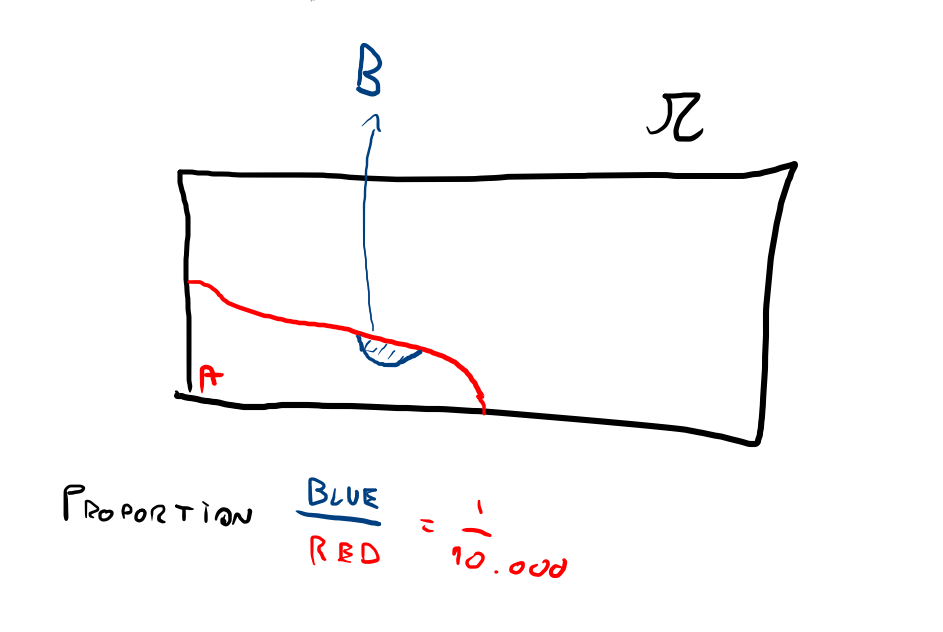
\includegraphics[width = 8cm]{Judicial_defence.png}
	    \caption{Defense argument: The proportion between the two areas is small }
	    \label{fig:defence}
	    \end{figure}
	    We wish to compute 
	$\mathbb{P}(B\vert A\cap(B\cup C))$, which, which is depicted in Figure ~\ref{fig:right}.
	\begin{figure}
	 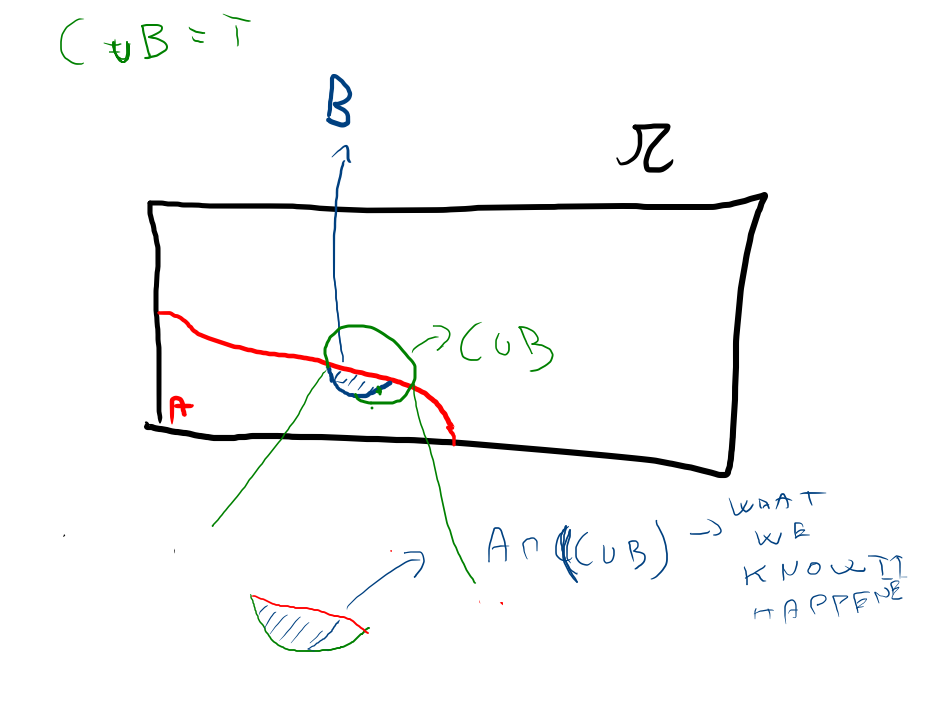
\includegraphics[width = 11cm]{Right.png}
	    \caption{What we need to compute: the proportion of the blue area with respect to the total area. Why this is what we need to compute is shown in \eqref{e:proportions} }
	    \label{fig:right}
	\end{figure}
	
	\bel{e:proportions}{\mathbb{P}(B\vert A\cap(B\cup C)) & =\frac{\mathbb{P}(B\cap A\cap (B \cup C)}{\mathbb{P}(A\cap (B\cup C))}=\frac{\mathbb{P}(B\cap A)}{\mathbb{P}((B\cup C)\cap A))}\\
	 &=\frac{\mathbb{P}(B\cap A)}{\mathbb{P}(B\cap A)+\mathbb{P}(C\cap A)}=\frac{1}{1 + \frac{\mathbb P(C \cap A)}{\mathbb P(B \cap A)}}.}
	Thus it is not $\mathbb{P}(B|A)$ that matters, but only its relative value $\mathbb{P}(B|A)/\mathbb{P}(C|A) = \mathbb P(C \cap A )/ \mathbb P (B \cap A)$, as shown in Figure ~\ref{fig:right}. We assume that $C$ and $A$ are independent, so that $\mathbb P(C|A) = \mathbb P(C)$ and \eqref{e:proportions} becomes 
	$$
	\mathbb P(B \vert A \cup ( B \cap C)) = \frac{1}{1 + \frac{\mathbb P(C)}{\mathbb P(B \vert A)}}.
	$$
	We estimate the $\mathbb P(C)$ by the probability that a woman gets killed: $\mathbb P(C) \leq \mathbb P(B \cup C)$
	which they estimated by  $\mathbb{P}(B\cup C)=1/100000$. Therefore \bel{}{\frac{\mathbb{P}(C|A)}{\mathbb{P}(B|A)}\leq 1/10.}
	Plugging in this value, one obtains that
	\bel{}{\mathbb{P}(B\vert A\cap(B\cup C))\geq 10/11}
	At the end, the man has been judged guilty. 
	
	
	
%%%%%%%%%%%%%%%%%%%%%%%%%%%%%%%%%%%%%%%%%%%%%%%%%%%%%%%%%%%%%%%%%%%%%%%%%%%%%%%%%%%%%%%%%%%%%%%%%%%%%%%%%%%%%%%%%%%%%%%%%%%%%%%%%%%%%%%%%%%%%%%%%%%%%%%%%%%%%%%%%%%%%%%%%%%%%%%%%%%%%%%%%%%%%%%%%%%%%%%%%%%%%%%%%%%%%%%%%%%%%%%%%%%%%%%%
%%%%%%%%%%%%%%%%%%%%%%%%%%%%%%%%%%%%%%%%%%%%%%%%%%%%%%%%%%%%%%%%%%%%% SAMPLING INTERPRETATION OF CONDITIONAL PROBABILITY %%%%%%%%%%%%%%%%%%%%%%%%%%%%%%%%%%%%%%%%%%%%%%%%%%%%%%%%%%%%%%%%%%%%%%%%%%%%%%%%%%%%%%%%%%%%%%%%%%%%%%%%%%%%%%%
%%%%%%%%%%%%%%%%%%%%%%%%%%%%%%%%%%%%%%%%%%%%%%%%%%%%%%%%%%%%%%%%%%%%%%%%%%%%%%%%%%%%%%%%%%%%%%%%%%%%%%%%%%%%%%%%%%%%%%%%%%%%%%%%%%%%%%%%%%%%%%%%%%%%%%%%%%%%%%%%%%%%%%%%%%%%%%%%%%%%%%%%%%%%%%%%%%%%%%%%%%%%%%%%%%%%%%%%%%%%%%%%%%%%%%%%
	
	\subsection{Independence of Events }
		\label{ss:independence}
		In view of the definition of condiitonal probability in Definition~\ref{d:conditional} the following definition is natural to say that the events $A$ and $B$ are independent if $\mathbb P(A) = \mathbb P(A| B)$. In a more symmetric form 
		\begin{definition}
			Two events $A, B \subset \Omega$ are \emph{independent} if  
			\bel{e:ind}{
				\mathbb{P}(A \cap B) = \mathbb {P}(A) \mathbb{P}(B).
			}
		\end{definition}
		It is important to notice that the word "independent" can be missleading, since it could be wrongly associated to the absence of a causal relation between $A$ and $B$. Example~\ref{ex:ind}  shows that there are events not related by any causal relation that are dependent and that, conversely, there are independent events that are causal. The events $A$ and $B$ are independent if from the knowledge of one of them you cannot infer anything on the evaluation of the probability of the other one: the probability remains the same. For this reason the independence property is sometimes stochastic independence. Another way to see that the notions of causality and independence are unrelated is by noting that the notion of independence depends from the probability $\mathbb P$, while the notion of causality does not. 
	


    Note that the notion of independence is unrelated with the notion of causality. The notion of causality is a notion that takes into account only the relation between events, while the notion of independence takes into account the notion of probability. Independence means that, given $\mathbb P$, that is, having an evaluation of the probabilities of the events, we can infer no information from the realization of $B$ that causes to change the evaluation of the probability of $A$. Thus is a probability dependent hypothesis and, for instance, Exercise \eqref{ex:coin} shows that coin tosses are not independent if we don't know exactly the parameter of the coin, since we can infer some information useful to determine the coin parameter by tossing the coin, which, in turn, will change the probability of the next toss. It is the same situation of \eqref{ex:indep}, which makes clear the striking fact that the number of shark attacks and the number of ice creams sold are numbers with a strong dependence, even if, of course, not related by any causal relation. 
    %Vice versa, if you toss twice a fair coin, the first toss changes the state of the room, molecules of air, \ldots  and therefore could change the output of the second coin toss, but it does it in such a way that the probability of the second toss will still be $1/2$. So the there is a "dependence" between the two tosses, but is so "caotic" that you cannot infer anything from it


\begin{example}[Two independent uniform samplings]
\label{example_fundamental}
Consider a bowl where 3 marbles, 1 red, 1 blue and 1 green, are placed and draw two marbles with replacement. The state space of the system is 
\bel{}{\Omega = \{(r,r),(r,b),...,(g,g)\},}
We want to prove that the following are equivalent: 
\begin{itemize}
 \item The probability measure on $\Omega$ is the uniform one. \\
\item In each single extraction you can draw each marble with the same probability and the extractions are independent
\end{itemize} 
To see what the second condition means precisely, let's assume that $\mathbb P$ is uniform and define the events 
\bel{}{
    F_c = \textrm{"The colour of the first marble is c"} = \{ (c,r), (c,b), (c,g)\},
}
for $c = r,b,g$, and  
\bel{}{
    S_c = \textrm{"The colour of the second marble is c"} = \{ (r,c), (b,c), (g,c)\},
}
for $c = r,g,b$. By saying that each extraction is a "random" extraction (that is, is uniform) we mean that 
\bel{1}{
 \mathbb P(F_c) =&  1/3\\
 \mathbb P(S_c) = & 1/3 
}
for each $c = b,g,r$, which is easily seen to hold true. By the fact that the extractions are independent we mean that for each $c$ and $c'$ in $\{r,b,g\}$
\bel{2}{
\mathbb P(F_c \cap S_{c'} ) = \mathbb P(F_c)\mathbb P(S_{c'})
.}
The event on the left hand side is the singleton $\{(c,c')\}$, so that its probability is $1/9$. The events on the right hand side have probability 1/3, so that the above equality holds. 
Let's assume that now \eqref{1} and \eqref{2} hold. Then 
\bel{}{\mathbb P(c,c') &= \mathbb P (F_c\cap S_{c'}) \\ & = \mathbb P(F_c)\mathbb P(S_{c'}) = 1/3 \times 1/3 = 1/9, }
so that $\mathbb P$ is uniform. This example will be generalised in Section \ref{s:two_experiments} to the case where the two extraction procedure can be performed jointly in an arbitrary way.  Examples \eqref{MountyHall} and Exercise \eqref{Prisoner} and \eqref{3cards} will show examples in which you perform two dependent extractions and how this can lead to surprising results.  
\end{example}

\begin{example}[Mounty Hall Problem]
\label{MountyHall} In a game show called the Mounty Hall, the participants had to choose between three doors. Behind 1 door there was a car while behind the other two there was a goat. The participant had to guess which door contained the car. After the first choice, the host disclosed a door which had behind a goat and then asked the participant  whether or not he would like to change the choice of the door. The result is at a first sight surprising. Let's call Strategy 1 the strategy in which we don't change the door, and Strategy 2 the strategy in which we decide to change the door. Then $\mathbb P(\textrm{"win"}) = 1/3$ if we play following Strategy 1, and $\mathbb P(\textrm{"win"}) = 2/3$ if we play by Strategy 2  \\
To prove the above fact, assume that the participant choses the door 1 and that he plays following Strategy 2. The result is clear if one observes that the participant wins if and only if he chooses a goat at the beginning. 
\textbf{Exercise:} Consider the Mounty Hall problem with n doors and  k cars. What is the probability of winning under Strategy 2? \\


\textbf{Solution} 
The sample space should encode the doors, the thing that is behind the door, the first door chosen by the participant and its second choice. However, we can give a reduced description since we are interested only on the choices the participant makes. The sample space can be taken to be $\Omega = \{ CC, GG,GC, CG\}$ where the first digit denotes what is there behind the first door and similarly for the second.
Let's denote the event 
"The first choice is a car"  by $F$, and the event "The second choice is a car" = "win" by $S$. Therefore 
\bel{}{\mathbb P(S) = \mathbb P(S|F) \mathbb P(F) + \mathbb P(S|F^c)\mathbb P(F^c),} 
but, given $F$, after the goat is revealed, the participant chooses between n-2 doors with k-1 cars. Given $F^c$, then, after the host reveals the goat, has to choose between $n-2$ doors and $k$ cars. Therefore 
\bel{}{\mathbb P(S) &= \mathbb P(S|F) \mathbb P(F) + \mathbb P(S|F^c)\mathbb P(F^c) \\
& = \frac{k-1}{n-2}\frac{k}{n} + \frac{k}{n-2}\frac{n-k}{n}} 
So, it is not diffiucult to understand the Mounty Hall problem: what happens is that the different extractions, the first door and the second one are dependent.  
\end{example}
The next "paradox" has interest on its own and shows that it is important to clearly state the conditioning event
\begin{example}[Boy or Girl Paradox ]
Consider a family with two children and consider their genders. The state space is $\Omega =\{MM,MF,FM,FF\}$ and consider the uniform probability on it. \sidenote{It is actually a little bit statistically more probable to have a daughter that a son.}

\begin{enumerate}

	\item What is the probability that the second child of a couple is a boy, knowing that the firs one is a boy?
	\item Assume that we get to know that one of the children is a boy. What is the probability that both children are males? 
	\item We have chosen a child randomly (and independently on the gender, of course) and have seen that he is male. What is the probability that both children are boys? (Note that the first poin is a particular case of this one, when the chosen child is surely the first one).

\end{enumerate}

For the first question, look at the sample space $\Omega=\{(M,M),(M,F),(F,M),(F,F)\}$ and endow it with the uniform probability ( see Example ~\ref{example_fundamental}).  The event A="The first child is male" is given by $\{(M,M),(M,F)\}.$ A basic computation shows that  $$\mathbb{P}((M,M)|A)=\mathbb{P}(M,M)/\mathbb{P}(A)=\frac{1/4}{2/4}=1/2.$$

As for the second question, maybe counterintuitively, the answer is  $1/3$. In this case the conditioning event $A$ is $\{(M,M),(M,F),(F,M)\}$, and 
\bel{}{\mathbb{P}((M,M)|A)=\mathbb{P}(M,M)/\mathbb{P}(A)=\frac{1/4}{3/4}=1/3.}
In the last case, the probability is $1/2$! Let's take as state space $\Omega=\{MM1,MM2,MF1,MF2,FM1,FM2,FF1,FF2\}$, where the last number means that you have observed the gender of the child 1 or child 2. The event A="you observed a male child"=$\{MM1,MM2,MF1,FM2\}$, while the event "The couple has two male children" is $B=\{MM1,MM2\}$. Since we assume that the choice is done independently, we have that if we denote 1=" I observed the first child"  $\mathbb{P}(MM1|1)=\mathbb{P}(MF1|1)=\mathbb{P}(FF1|1)=1/4$. Similarly for the event 2 = "I observed the second child ". We assuem that $\mathbb{P}(1)=p$ and we compute 
\bel{}{ \mathbb{P}(A) = \mathbb{P}(\{MM1,MF1\}|1)\mathbb{P}(1)+ \mathbb{P}(\{MM2,FM2\}|2)\mathbb{P}(2) = p/2+(1-p)/2=1/2, }
and 
\bel{}{\mathbb{P}(\{ MM1,MM2\}) =\mathbb{P}(MM1|1)\mathbb{P}(1)+\mathbb{P}(MM2|2)\mathbb{P}(2) = 1/4. }
\bel{}{
	\mathbb{P}(\{MM1,MM2\}|A)=\mathbb{P}(A \cap B) / \mathbb{P}(A) = 1/2.}

 Even if the second point of the example might come as a surprise, if one interprets the probability with a wrong frequentist definition, if one were to obtain the list of all the families with two children such that one is a male, then approximately 1/3 of the hamilies in those lists will have 2 male children. The procedure 3 would have the following equivalent in the frequentist approximation. From the list of all the families with two children, you toss an unfair coin to decide which children to take into account and to check. So there is a 

\end{example}

\begin{ExerciseList}

	\Exercise You toss a fair coin 4 time.Assume that every outcome is equally probable ( we will rigorously see why ). Show that the events "The fourth toss gave heads" and the event "The first three tosses gave head" are independent.  

	\Exercise In the setting of Example ~\ref{example_fundamental} you draw two marbles without replacement.
    \Question What are the probabilities of each single extraction? 
    \Question Are extractions independent? 
	
	\Exercise
    \label{ex:3indep}
    $\Omega = \{1,2,3,4\}$ and $\mathbb{P}(i) = 1/4 $ for every $i\in \Omega$. Show that $A=\{1,2\}$ $B=\{1,3\}$ and $C=\{2,3\}$ are pairwise independent but not independent. 

    \Exercise 3 prisoners, (A,B,C) are condemned to death. They decide to save one of them, but the name will be given only some minutes before the executions. A asks to a guard if he will be saved, but gets no answer. A asks then which one between B and C will be executed, and the guard says C. At this point A says."Now only one between me and B will be executed; I have 50\% of chances to survive ". Is it correct his reasoning?

%	\Answer Is the same situation as the one in the above example: you are not asking if $C$ will or not will be executed. The guard is telling you which one between $B$ and $C$ will be executed, and you don't know why he has chosen $C$. If you have no information on why the guard would tell you  about the execution of $C$ instead f the execution of $B$, wen both have to be executed, then the probability that $A$ is executed is still $1/3$. 
%	To see this consider the sample space$ \{(AB,B), (AC,C), (BC,B), (BC,C)\}$, where the first component tells who will be executed and the second who the guard says it will be. Denote the events that the guard tells that $B$ will be  executed and the durd tells that $C$ will be executed by GB and GC respectively. We assume that when $BC$= "both B and C will be executed" happens, the guard tells $B$ or $C$ according to some probability $\mathbb{P}(GC| AB)$. We are looking for the probability of the event $A=\{(AC,C), (AB,B)\}$ that prisioners B and C will be excecuted, given $GC$. We use the total probability formula to get 
%
%	\bel{}{\mathbb{P}(GC)=\mathbb{P}(GC|AC)\mathbb{P}(AC)+\mathbb{P}(GC|BC)\mathbb{P}(BC)=1/3+1/3\mathbb{P}(GC|BC),}
%and that
%	\bel{}{\mathbb{P}((AC,C))=\mathbb{P}(GC|AC)\mathbb{P}(AC)=1/3,}
%	so that, finally 
%	\bel{}{\mathbb{P}(A|GC) = \mathbb{P}(AC|GC) & =\frac{\mathbb{P}((AC,C))}{\mathbb{P}(GC)} =  \\
%	 & = \frac{1/3}{1/3+1/3\mathbb{P}(GC|BC)}.}
%	$\mathbb{P}(GC|BC) =1/2 $, the above value is $2/3$ and the event A is indipendent from the event GC.
%
\Exercise There are three cards one of them has both faces black, one with both red faces, and the last one with one black face and the other face red. You draw a card and observe a red face. What is the probability that the other face is red? 

%\Answer
%	Denote by A  the event "I observe a red face". Clearly $\mathbb{P}(A)=1/2$. Let B="The other side is red" and observe that $A\cap B$= "I draw the red red card". $\mathbb{P} ( A\cap B) = 1/3.$
%	\bel{}{\mathbb{P}(B|A)=\frac{\mathbb{P}( B \cap A)}{\mathbb{P}(A)}= \frac{1/3}{1/2}=2/3.}
%	If you want you can introduce the sample space of $\Omega=\{(RR,R),(RB,R),(RB,B), (BB,B)\}$, where the first component denotes the extracted card and the second one the shown face, andyou can repeat the same computations. 
%
\end{ExerciseList}

This example shows that is important to clearly state the conditioning event. 

\begin{enumerate}

	\item What is the probability that the second child of a couple is a boy, knowing that the firs one is a boy?
	\item We know that one of the child is a boy. What is the probability that both children are males? 
	\item We have chosen a child randomly (and independently on the gender, of course) and have seen that he is male. What is the probability that both children are boys? (Note that the first poin is a particular case of this one, when the chosen child is surely the first one). 

\end{enumerate}

For the first question, look at the sample space $\Omega=\{(M,M),(M,F),(F,M),(F,F)\}$ and endow it with the uniform probability ( in section \ref{} we will see that this is due to the fact that we regard rhe gender of the two child as independent, and the probability of each single child to be either a boy or a girl 1/2). The event A="The first child is male" is given by $\{(M,M),(M,F)\}.$ We are interested in $$\mathbb{P}((M,M)|A)=\mathbb{P}(M,M)/\mathbb{P}(A)=\frac{1/4}{2/4}=1/2.$$

Maybe counterintuitively, the answer is  $1/3$. But this is clear since the conditioning event $A$ is $\{(M,M),(M,F),(F,M)\}$, and 
\bel{}{\mathbb{P}((M,M)|A)=\mathbb{P}(M,M)/\mathbb{P}(A)=\frac{1/4}{3/4}=1/3.}
Using a frequentist approach, if one had the list of al the couples with two children, one of which male, approximately $1/3$ would have two male childeren.\\  
In the last case, the probability is $1/2$! Let's take as state space $\Omega=\{MM1,MM2,MF1,MF2,FM1,FM2,FF1,FF2\}$, where the last number means that you have observed the gender of the child 1 or child 2. The event A="you observed a male child"=$\{MM1,MM2,MF1,FM2\}$, while the event "The couple has two male children" is $B=\{MM1,MM2\}$. Since we assume that the choice is done independently, we have that if we denote 1=" I observed the first child"  $\mathbb{P}(MM1|1)=\mathbb{P}(MF1|1)=\mathbb{P}(FF1|1)=1/4$. Similarly for the event 2 = "I observed the second child ". We assuem that $\mathbb{P}(1)=p$ and we compute 
\bel{}{ \mathbb{P}(A) = \mathbb{P}(\{MM1,MF1\}|1)\mathbb{P}(1)+ \mathbb{P}(\{MM2,FM2\}|2)\mathbb{P}(2) = p/2+(1-p)/2=1/2, }
and 
\bel{}{\mathbb{P}(\{ MM1,MM2\}) =\mathbb{P}(MM1|1)\mathbb{P}(1)+\mathbb{P}(MM2|2)\mathbb{P}(2) = 1/4. }
\bel{}{
	\mathbb{P}(\{MM1,MM2\}|A)=\mathbb{P}(A \cap B) / \mathbb{P}(A) = 1/2.}
This apparent paradox is due to the fact that the event $A$ is different from the event B="There is at least one male child". If you repeat the same calculations with $B$ instead of $A$, you should obtain $1/3$. 


You can interpret this example as the fact that is important to know how to get the information and it is important to specify the conditioning event rigorously. 

\begin{definition}
    Three events $A$,$B$ and $C$ are independent if they are pairwise independent  
    \bel{}{
    \mathbb{P}(A \cap B) &  =\mathbb{P}(A)\mathbb{P}(B), \\ \mathbb{P}(A \cap C)& =\mathbb{P}(A)\mathbb{P}(C),\\
    \mathbb{P}(B \cap C) & =\mathbb{P}(B)\mathbb{P}(C),
    } 
    and 
    \bel{}{\mathbb{P}(A\cap B \cap C)=\mathbb{P}(A)\mathbb{P} (B)\mathbb{P}(C).}
    
    \end{definition}
    An example three events that are pairwise independent but not independent is given in Exercise ~\ref{ex:3indep}. 

	\subsection{Sampling Interpretation of Conditional Probability}
		\label{ss:r_cond}
	We now come back to the example of Subsection~\ref{ss:r_prob}, where $\Omega = \{\omega_1, \ldots, \omega_6\}$ and we assume that we observe $E = \{\omega_1, \omega_4, \omega_5, \omega_6\}$. We can define the conditional probability by setting $p_2 = p_3 = 0$ and normalising the thuis obtained vector so that the sum is 1.

%<<label=hello>>=
%n <- 6  # The number of elements of our sample space
%Omega <- paste("omega",1:n) # Here I define the sample space, and I give to its elements the names omega_i, for i =1,...,n
% p_aux <- c(1,2,3,0.5,1,5) # Here I take the p_i to be positive numbers whose sum needs not to be 1 
%p <- p_aux/sum(p_aux) # Now I normalise them so that they sum 1
%#E = paste("omega", as.char(c(1,4,5,6)))
%p_cond = 
%sample(Omega, 1, prob = p_cond  ) # The output of the sample
%@
	Looking at Example~\ref{ex:sampling_cond}, if we know how to sample from $\mathbb P$, and indeed we were able to do it in Subsection~\ref{ss:r_prob}, we can sample from the $\mathbb P()$ 
%<<>>=
%x <- sample(Omega, p) # We obtain an omega_i with probability $p_i$
%while(x !in E ){
%x <- sample(Omega, p)
%}
%@
%%	

	\subsection{Total probability Formula}

When speaking about events many times one reasons by cases in the following sense. Assume you don't know whwther to go out this night, then, in order to think at the event "I will go out this night" one thinks at this event first in the case it rains, then in the case it is good weather. Since the probability is simply a quantitative version of the logic we use when speaking about  events, we might hope to reproduce the same reasoning at the  quantitative level of probabilities. This is indeed true and it is done in the Total Probability Formula.
\begin{proposition}[Total Probability Formula for two conditioning events]
Let $B\subset \Omega$ be an event such that $\mathbb P(B) \in (0,1)$. Then 
\bel{e:totaleasy}{\mathbb{P}(A)=\mathbb{P}(A|B)\mathbb{P}(B)+\mathbb{P}(A|B^c)\mathbb{P}(B^c)}
\end{proposition}
\begin{proof}
\bel{}{\mathbb{P}(A)=\mathbb{P}(A\cap\Omega)=\mathbb{P}(A\cap(B\cup B^c))=\mathbb{P}((A\cap B)\cup (A\cap B^c)).}
Since $A\cap B$ and $A\cap B^c$ are disjoint, we can use the \eqref{e:add} to develope the above expression into 
\bel{}{\mathbb{P}(A)& =\mathbb{P}(A\cap B)+\mathbb{P}(A\cap B^c)=\frac{\mathbb{P}(A\cap B)}{\mathbb{P}(B)}+\frac{\mathbb{P}(A\cap B^c)}{\mathbb{P}(B^c)}\\ &=\mathbb{P}(A|B)\mathbb{P}(B)+\mathbb{P}(A|B^c)\mathbb{P}(B^c),}
which is what we wanted to prove.
\end{proof}

\begin{ExerciseList}
    
\Exercise We toss a fair coin. If the coin gives heads we draw a ball from a bowl that contains a blue ball, a red ball and a white ball. If the con gives tails, we draw a ball from a bowl that contains a blue ball or a red ball. What is the probability of drawing a red ball?

\Answer Let's call B="The coin gave heads". We know that $\mathbb{P}(B)=\mathbb{P}(B^c)=1/2$. We also know that the event r=" We draw a red ball" has the following probabilities conditioned on $B$:
\bel{}{\mathbb{P}(r|B)=1/3,\,\,\mathbb{P}(r|B^c)=1/2.}
We can apply formula \eqref{e:totaleasy} to obtain 
\bel{}{\mathbb{P}(r)=\mathbb{P}(r|B)\mathbb{P}(B)+\mathbb{P}(r|B^c)\mathbb{P}(B^c)=1/2\cdot 1/3+1/2\cdot 1/2=5/12.}

\end{ExerciseList}


We now give the total probability formula in full generality. The proof is almost the same, but we need to introduce the concept of partition of the sample space $\Omega$:
\begin{definition}
The events $B_1$,...,$B_n$ are said to be mutually disjoint if $B_i\cap B_j=\emptyset$ whenever $i\neq j$.
A partition is a set $\{B_1,...,B_n\}$ of mutually disjoint events $B_i$, such that $\Omega=\bigcup_{i=1}^n B_i$.  
\end{definition}
Examples of partitions are 
\begin{itemize}
    \item In 4 coin tosses, a partition of $\Omega=\{0000,0001,....,1111\}$ in two events is, for example, $\{B_1,B_2\}$, where $B_1$="The first toss gave tail" and $B_2=(B_1)^c$="The first toss was head". Another partition would be $\{C_0,C_1,C_2,C_3,C_4\}$ where $C_i= "\textrm{There have been $i$ heads}"$. 
    \item In the roll of a die, an example of partition of $\Omega=\{1,2,3,4,5,6\}$ is 
    $\{B_1,B_2\}$, where $B_1=\{2,4,6\}=$"The result is an even number", and $B_1=\{1,3,5\}=$"The result is an odd number".
    \item If we roll two dice, a partition is $\{B_2,...,B_{12}\}$, where $B_i$ is the event "The sum of the dice is i".
	    	\item We observe some coin tosses but we don't know how many of them there will be. Thus $\Omega$ is the one given by \eqref{d:finite_coin} and it can be partitioned into $\Omega = \cup_n \Omega_n$, where $\Omega_n$=" There have been $n$ tosses "$=\{x_1...x_n\,,x_i\in\{0,1\}\}$.  
\end{itemize}

In other words a partition is a family of mutually disjoint events (or hypotheses) that together they include all the possible eventualities, conditions intuitive and necessary to make reasonings of the form " If $B_1$, then    and you can reason separately on each element of the partition, both at the level of sets and at the level of probabilities thanks to the next
Note that if a partition consists of two events $B_1$ and $B_2$, then $B_2=(B_1)^c$. 

\begin{proposition}[Total probability formula]
Let $\{B_1,....,B_n\}$ be a partition of $\Omega$. Then 
\bel{}{\mathbb{P}(A)=\mathbb{P}(A|B_1)\mathbb{P}(B_1)+...+\mathbb{P}(A|B_n)\mathbb{P}(B_n).}
\end{proposition}
We omit the prove, which is similar to the previous and we remark that, up to some basic knowledge of series, one could take a partition to be an infinite family of the form $\{B_i\}_{i \in \mathbb N}$, and the total probability formula would still be true. 

\begin{ExerciseList}

	\Exercise Consider an infection that is contagious and which is suffers by 1 person out of  1000.  There is a test used to determine whether a person has the infection and the test has a 5\% of possibility of giving a false positive: You don't have the infection but the test is positive, while the probability of having a false negative is zero.  
	\Question If you are tested positive, what is the probability of actually having the infection? 
	\Question You have some symptoms and the doctors estimate around 50\% of probability that you have the infection. What is the probability that you have the infection provided that the test gives a positive result? 
%	\Answer 
%	Let the sample space be $\{(C,P), (C,N), (NC,P), (NC,N)\}$, where $C$ tells you that you have covid and NC that you dont.  The second variable is the result of the test. 
%	\Question For the first question, the data that is given to you is, denoting A="You tested positive", B="you have covid", is that $\\mathbb{P}(B)=1/1000$, that $\mathbb{P}(A|B)= 1$ and that $\mathbb{P}(A|B^c)=5/100$. You are interested in 
%	$\mathbb{P}(B|A)$ 
%	\bel{}{\mathbb{P}(B|A) = \frac{\mathbb{P}(A \cap B)}{\mathbb{P}(A)} = \frac{\mathbb{P}(A|B) \mathbb{P}(B)}{\mathbb{P}(A)}  }
	
%	The only information that is left is $\mathbb{P}(A)$. We use the total probability formula 
%	\bel{}{\mathbb{P}(A)=\mathbb{P}(A|B) \mathbb{P}(B)+ \mathbb{P}(A|B^c)\mathbb{P}(B^c) = \mathbb{P}(A|B)\mathbb{P}(B),}

%	\bel{}{\mathbb{P}(B|A) = \frac{\mathbb{P}(A|B) \mathbb{P}(B)}{\mathbb{P}(A)}  }
	
%	\Question Doing the same computations, now using $\mathbb{P}(B) = 50/100$, shows that the probability now is much higher. 

%	\commento{The reason is that even if the test has a good presition, on 1000 people the positive tests come 1 from a person that effectively has covid, while the other 999 x 5\% $\sim$ 50 come from  of a false positive. Around 1/51  is the proportion of the people with covid in the population of  }
%	Put an image here!!


 \Exercise \label{ex:indep} We have two urns, one containing $3$ red balls, $1$ blue ball, and one white ball, the other one containing 3 blue balls, 1 red ball and 1 white ball. We toss a fair coin to choose one of the two urns. 
    \Question We draw a ball from the chosen urn. What is the probability that you extract a red ball? (Hint: Use the total probability formula)
    \Question Now we extract a ball, reinsert it in the urn, and draw again another ball from the same urn. Are the event "The first ball extracted is red" and the event "The second  ball  extracted is red" independent? 
    

% \commento{This exercise shows that independence is much more general than causality. Causality is a property of the events, while independence is a property of the probability $\mathbb{P}$. The fact that the events $A$ and $B$ are independent tells you that from the knowledge of $B$ you cannot infer anything that changes the probability of $A$. Think at this example: A = "The number of sharks attacks this week in Spain is 4" and B=" The number of ice-creams sold this week in a shop is of 4.000" are not related by any causality relation but they are dependent! 4 shark attacks is a huge number, and if it happens you can infer that  is more likely that it is summer. Thus also the event $B$ is more likely. It is the same of what happens above: You draw a red ball, then it is more likely that the coin gave heads, and then it is more likely that you draw a second time a red ball.   }


  %  \sidenote{ This is really similar to the previous exercise, which can be thought as an urn about whose composition you are uncertain. But somehow it makes even more evident that independence is a notion of inference.}

\end{ExerciseList}

\subsection{Odds and Bayes Formula}

